\documentclass[letterpaper,10pt]{article}
\usepackage[top=2cm, bottom=1.5cm, left=1cm, right=1cm]{geometry}
\usepackage{amsmath, amssymb, amsthm,graphicx}
\usepackage{fancyhdr}
\pagestyle{fancy}

\lhead{\today}
\chead{MATH 710 Assignment 3}
\rhead{Justin Hood}

\newcommand{\Z}{\mathbb{Z}}
\newcommand{\Q}{\mathbb{Q}}
\newcommand{\R}{\mathbb{R}}
\newcommand{\C}{\mathbb{C}}
\newtheorem{lem}{Lemma}

\begin{document}
\begin{description}
\item[Page 330]\hfill\\
\begin{enumerate}
\item Find the first four terms of the solutions to the following difference equations.
\begin{enumerate}
\item $x(t+1)-x(t)=x(t)^2+t$, $x(0)=1$
\begin{align*}
x(0)&=1\\
x(1)&=2\\
x(2)&=7\\
x(3)&=58\\
x(4)&=3425
\end{align*}
\item $x(t+1)-x(t)=t^2+t+1$, $x(0)=-1$
\begin{align*}
x(0)&=-1\\
x(1)&=0\\
x(2)&=3\\
x(3)&=10\\
x(4)&=23
\end{align*}
\item $x(t+1)-x(t)=\frac{t}{x(t)}$, $x(0)=1$
\begin{align*}
x(0)&=1\\
x(1)&=1\\
x(2)&=2\\
x(3)&=3\\
x(4)&=4
\end{align*}
\end{enumerate}
\item Consider the equation,
\[x(t+1)-x(t)=a,\ x(0)=b\]
For arbitrary $a$ and $b$. We examine some terms of the solution as follows.
\begin{align*}
x(0)&=b\\
x(1)&=x(0)+a=a+b\\
x(2)&=x(1)+a=2a+b\\
\vdots\\
x(t)&=at+b
\end{align*}
Thus, we see that $at+b$ is the general solution to the difference equations.
\item \hfill \\
\begin{enumerate}
\item Plot the solutions to $x(t+1)-x(t)=1$ for the initial conditions, $x(0)=-1,0,1$
\begin{center}
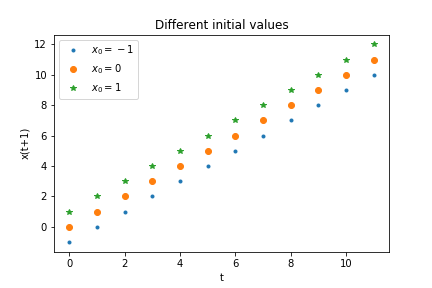
\includegraphics[scale=.7]{intl.png}
\end{center}
We see that these solutions all share the same slope, 1, regardless of the initial conditions of the system.
\item We now plot the solutions to  $x(t+1)-x(t)=a$ with initial condition $x(0)=1$ and constants $a=-1,0,1$
\begin{center}
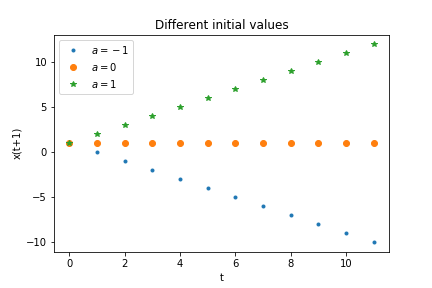
\includegraphics[scale=.7]{const.png}
\end{center}
We see that this time, the solutions all start at the same point, but the differing values of $a$ provide different slopes to the solution sets.
\end{enumerate}
\addtocounter{enumi}{1}
\item \hfill\\
\begin{enumerate}
\item Consider the equation, $x(t+1)-x(t)=-2x(t)$ with initial condition $x(0)=3$. We will solve as follows:
\begin{align*}
x(t+1)&=-x(t)\\
x(t+2)&=-x(t+1)\\
x(t+3)&=-x(t+2)=-(-x(t+1))\\
x(t+4)&=-x(3)=-(-(-x(t+1)))\\
\vdots\\
x(t)&=(-1)^tx(0)=(-1)^t(3)
\end{align*}
We shall now check our solution by substitution,
\begin{align*}
x(1)&=-3=(-1)^1x(0)\\
x(2)&=3=(-1)^2x(0)\\
x(3)&=-3=(-1)^3x(0)\\
\vdots
\end{align*}
\item We now do the same for the equation $x(t+1)-x(t)=kx(t)$ with initial condition $x(0)=a$.
\begin{align*}
x(t+1)&=(k-1)x(t)\\
x(t+2)&=(k-1)x(t+1)=(k-1)(k-1)x(t)\\
x(t+3)&=(k-1)x(t+2)=(k-1)(k-1)(k-1)x(t)\\
\vdots\\
x(t)&=(k-1)^tx(0)=(k-1)^ta
\end{align*}
We shall now check our solution by substitution,
\begin{align*}
x(1)&=(k-1)a=(k-1)^1x(0)\\
x(2)&=(k-1)(k-1)a=(k-1)^2x(0)\\
x(3)&=(k-1(k-1)a=(k-1)^3x(0)\\
\vdots
\end{align*}
\end{enumerate}
\item Show that the solution to $x(t+1)-x(t)=x(t)^2+1$ with $x(0)=a,\ a>0$ has all terms positive.\\
We begin by manipulating the equation to have the form,
\[x(t+1)=x(t)^2+x(t)+1\]
Now, we consider the zeros of the equation,
\[x(t)^2+x(t)+1=0\]
Checking the discriminant, we see that $d=\sqrt{1^2-4(1)(1)}\in\C$ Thus, we know that there are no real roots of this system. So the values of the equation are either strictly positive or strictly negative. So it suffices to test a general $a$ term and compute $x(1)$. Consider $a=1$,
\[x(1)=1^1+1+1=3>0\]
Thus, we see that the values of this system are strictly positive.
\end{enumerate}
\item[Page 338]\hfill \\
\begin{enumerate}
\item Suppose 20 percent of a yeast population splits in any 15 minute interval. If 1 time unit designates 2 hours, what formula connects $x(t+1)-x(t)$ to $x(t)$.\\
We consider the following steps,
\begin{align*}
x(t+\frac{1}{8})&=1.20x(t)\\
x(t+\frac{1}{4})&=1.20x(t+\frac{1}{8})=1.20^2x(t)\\
x(t+\frac{3}{8})&=1.20x(t+\frac{1}{4})=1.20^3x(t)\\
\vdots\\
x(t+1)&=1.20^8x(t)
\end{align*}
Thus,
\[x(t+1)-x(t)=(1.20^8-1)x(t)\approx 3.2998x(t)\]
\addtocounter{enumi}{6}
\item Suppose a bank gives 5\% interest a year starting one year after deposit. Suppose you start with $M(0)=\$1000$.\\\\
Consider,
\begin{align*}
M(t+1)&=1.05M(t)\\
M(t+2)&=1.05M(t+1)=1.05^2M(t)\\
\vdots\\
M(t)&=1.05^t1000
\end{align*}
Thus,
\[M(t+1)-M(t)=(1.05^t-1)M(t)\]
\item Suppose now that the bank gives interest $n$ times a year in the amount of $.05/n$ for $n$ periods.\\\\
Consider,
\begin{align*}
M(t+\frac{1}{n})&=(1+\frac{.05}{n})M(t)\\
M(t+\frac{2}{n})&=(1+\frac{.05}{n})^2M(t)\\
\vdots\\
M(t+1)&=(1+\frac{.05}{n})^nM(t)\\
M(t)&=(1+\frac{.05}{n})^{nt}M(0)
\end{align*}
Thus,
\[M(t)=((1+\frac{.05}{n})^{nt})1000\]
Taking the limit as $n\to\infty$, we see that,
\[M(t)=e^{0.05t}M(0)\]
\end{enumerate}
\item[3.] We now consider the IVP,
\begin{align*}
\frac{dy}{dt}&=y\bigg(1-\frac{y}{3}\bigg)\\
y(0)&=y_0
\end{align*}
To better understand this system, we will conduct a basic stability analysis to compute the steady states for this IVP and their respective stabilities. First,
\[y\bigg(1-\frac{y}{3}\bigg)=0\Rightarrow y=0,3\]
Thus, our two stable states for this IVP are $0$ and $3$. Computing now we find the next derivative.
\[\frac{d^2y}{dt^2}=1-\frac{2y}{3}\]
With this information, we compute the following equalities,
\begin{align*}
\ddot{y}(0)>0\Rightarrow \text{Unstable}\\
\ddot{y}(3)<0\Rightarrow \text{Stable}
\end{align*}
Thus, we see that solutions with $y_0>3$ will tend down towards the stable state at $3$. Solutions with $0<y_0<3$ will tend up towards the stable state at $3$. Solutions with $y_0<0$ will tend away from the stable state towards $-\infty$. Thus, we shall pick an initial condition from each of these categories to test on our slope field. Consider $y_0=4,1,-.005$. We shall use Eulers method to solve the IVP numerically as,
\[y_n=y_{n-1}+\Delta t\frac{dy}{dt}\bigg|_{y_{n-1}}\]
The resultant slope field and solution curves are shown below.
\begin{center}
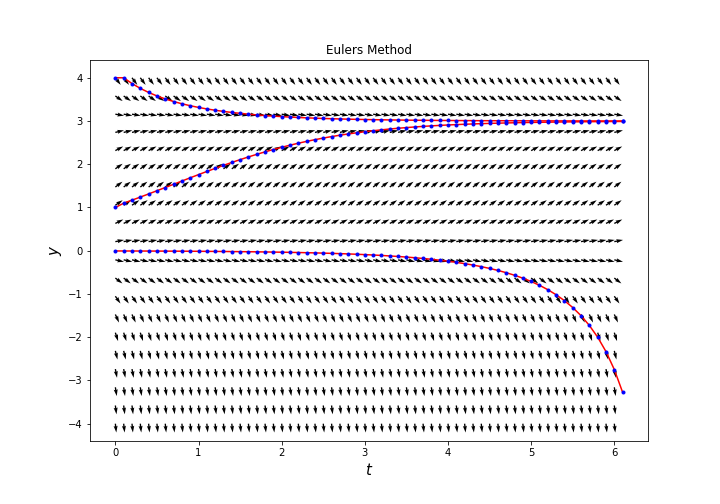
\includegraphics[scale=.7]{euler.png}
\end{center}
Here we see that the solutions behave as we would expect.
\item[4.] Finally, we consider the IVP,
\begin{align*}
\dot{y}&=(4-y)(2-y)^3\\
y(0)&=y_0
\end{align*}
As before, we will conduct a basic stability analysis for the equation. First,
\[(4-y)(2-y)^3=0\Rightarrow y=2,4\]
Thus, our two stable states for this problem are $2$ and $4$. We now evaluate,
\[\ddot{y}\big|_{2,4}\]
Hence, $\ddot{y}(2)=0,\ \ddot{y}(4)=8$. From this, we may conclude that the steady state at $4$ is unstable, but the state at $2$ requires further investigation. To find the stability for this point, we consider the following equalities,
\begin{align*}
\dot{y}(t)&>0,\ t\in(-\infty,2)\\
\dot{y}(t)&<0,\ t\in(2,4)
\end{align*}
From this, we may see that the slope field converges on the stable state from both sides of the value, so we note that it is a stable equilibrium.\\
Based on this analysis, we shall pick an initial condition from each of these categories to analyze on our slope field. Consider $y_0=1,3,5$. We shall use the Runge-Kutta method of order 4 to numerically solve the solutions and overlay them onto the appropriate slope field as seen below.
\begin{center}
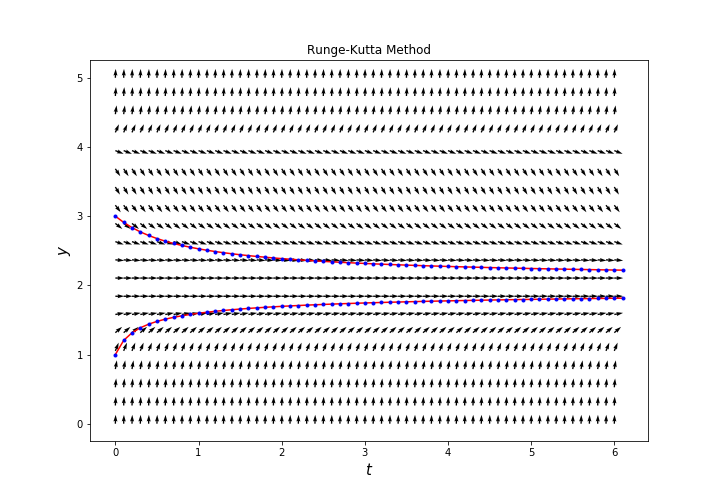
\includegraphics[scale=.7]{runge.png}
\end{center}
We see in this picture that the solution curve for $y_0=5$ is omitted, as the solution grows so quickly that we reach an overflow error over the relevant time interval. This is in line with our previous computation regarding the unstable nature of the equilibrium point at $4$.
\end{description}
\end{document}
